\documentclass{article}
\usepackage{amsmath}
\usepackage{tikz}
\usetikzlibrary{automata}
\usetikzlibrary{positioning, arrows}
\begin{document}
\textbf{Exercise 1}.

The determinization of the given NFA: (I literally tried my best.)
\begin{center}
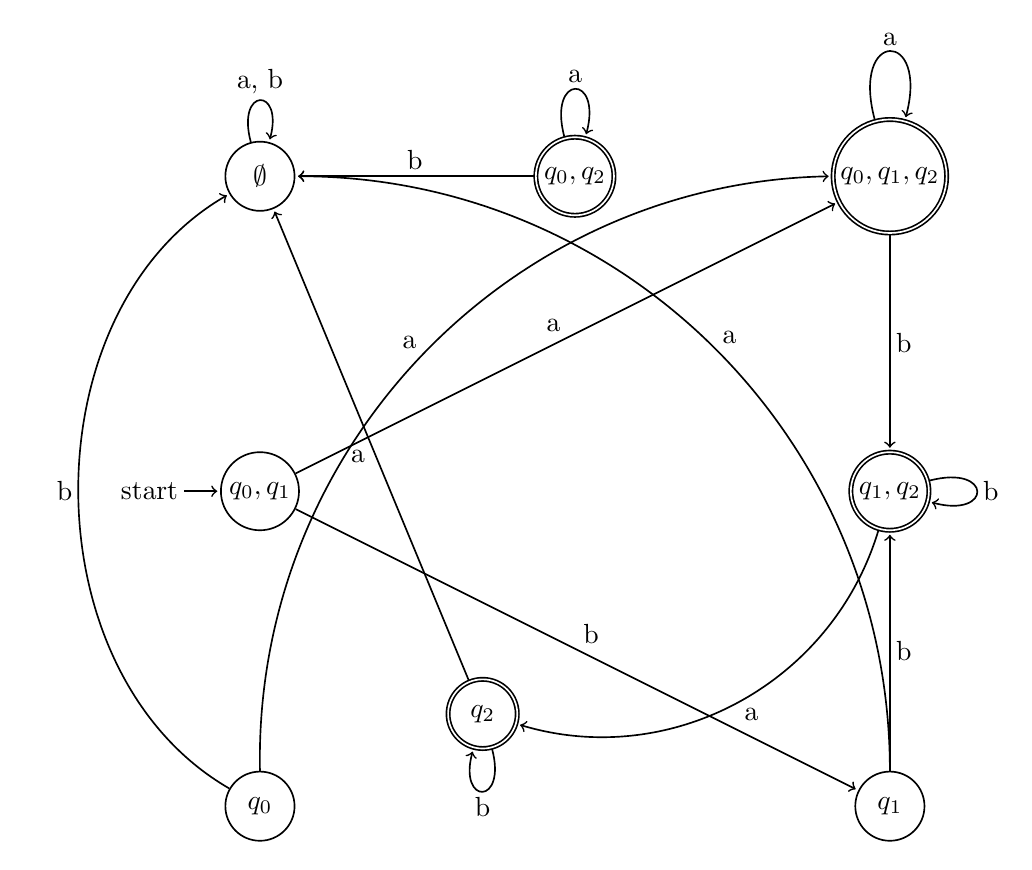
\begin{tikzpicture}
[->,shorten >=1pt,
                    auto,node distance=4cm,on grid,semithick,
                    inner sep=2pt,bend angle=45]
\node[state, initial] (q0q1) {$q_0, q_1$};
\node[state, above of=q0q1] (null) {$\emptyset$};
\node[state, accepting, right of=null] (q0q2) {$q_0, q_2$};
\node[state, accepting, right of=q0q2] (q0q1q2) {$q_0, q_1, q_2$};
\node[state, accepting, below of=q0q1q2] (q1q2) {$q_1, q_2$};

\node[state, accepting, below right of=q0q1] (q2) {$q_2$};
\node[state, below of=q1q2] (q1) {$q_1$};
\node[state, below of=q0q1] (q0) {$q_0$};

\path[->]
	(null) edge [loop above] node {a, b} ()
	(q1q2) edge [bend left] node {a} (q2)
		edge [loop right] node {b} ()
	(q0q1q2) edge [loop above] node {a} ()
		edge node {b} (q1q2)
	(q0q2) edge [loop above] node {a} ()
		edge node [swap] {b} (null)
	(q2) edge [loop below] node {b} ()
		edge node  {a} (null)
	(q1) edge [bend right] node [swap] {a} (null)
		edge node [swap] {b} (q1q2)
	(q0) edge [bend left] node {a} (q0q1q2)
		edge [bend left=60] node {b} (null)
	(q0q1) edge node {a} (q0q1q2)
		edge node {b} (q1);

	
\end{tikzpicture}
\end{center}

\textbf{Exercise 2}.

Here I'm going to trim it so you can actually make some sense of it :) (and also because I have to)

I moved $q_2$ to make the diagram a little simpler.

\begin{center}
\begin{tikzpicture}
[->,shorten >=1pt,
                    auto,node distance=2cm,on grid,semithick,
                    inner sep=2pt,bend angle=60]
\node[state, initial] (q0q1) {$q_0, q_1$};
\node[state, above of=q0q1] (null) {$\emptyset$};
\node[state, accepting, right of=q0q2] (q0q1q2) {$q_0, q_1, q_2$};
\node[state, accepting, below of=q0q1q2] (q1q2) {$q_1, q_2$};

\node[state, accepting, above of=null] (q2) {$q_2$};
\node[state, below of=q1q2] (q1) {$q_1$};

\path[->]
	(null) edge [loop left] node {a, b} ()
	(q1q2) edge node [swap] {a} (q2)
		edge [loop right] node {b} ()
	(q0q1q2) edge [loop above] node {a} ()
		edge node {b} (q1q2)
	(q2) edge [loop left] node {b} ()
		edge node [swap] {a} (null)
	(q1) edge node [swap] {a} (null)
		edge node [swap] {b} (q1q2)
	(q0q1) edge node {a} (q0q1q2)
		edge node {b} (q1);

	
\end{tikzpicture}
\end{center}
\textbf{Exercise 3}

\begin{center}
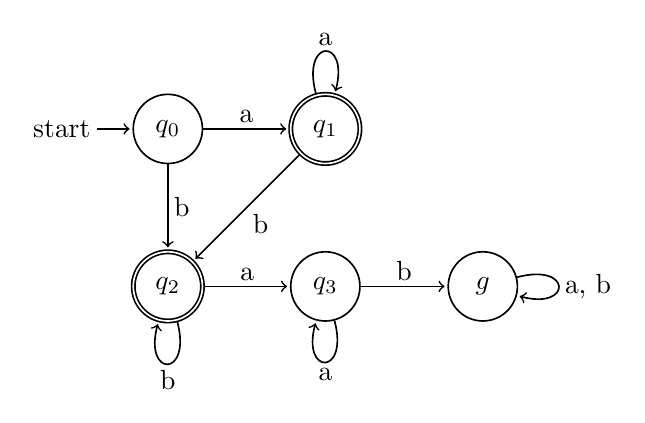
\begin{tikzpicture}
[->,shorten >=1pt,
                    auto,node distance=2cm,on grid,semithick,
                    inner sep=2pt,bend angle=45]
\node[state, initial] (q0) {$q_0$};
\node[state, accepting, right of=q0] (q1) {$q_1$};
\node[state, accepting, below of=q0] (q2) {$q_2$};
\node[state, right of=q2] (q3) {$q_3$};
\node[state, right of=q3] (g) {$g$};

\path[->]
	(q0) edge node {a} (q1)
		edge node{b} (q2)
	(q1) edge [loop above] node {a} ()
		edge node {b} (q2)
	(q2) edge node {a} (q3)
		edge [loop below] node {b} ()
	(q3) edge [loop below] node {a} ()
		edge node {b} (g)
	(g) edge [loop right] node {a, b} ();
\end{tikzpicture}
\end{center}


To show that there is no DFA with strictly fewer states that recoginzes $L(\mathcal{A})$, we attempt to minimize it. If the minimized DFA is the same, then we know there is no DFA with fewer states that recognizes the same language.

We know the given DFA is trimmed because no states are inaccessible. So we must determine whether any of the states are indistinguishable. The only two states we have that have the same residual language are $q_0$ and $q_1$. They would be indistinguishible, however $q_0$ is not final, whereas $q_1$ is. The rest of the states do not share residual languages, which means all of the states are distinguishible. Since all of the states are distinguishable, the minimization of $\mathcal{A}$ would have the same number of states as $\mathcal{A}$. Since a minimization is inherently unique, and the amount of states is by definition minimal, there is no DFA with strictly fewer states than $\mathcal{A}$ that recognizes $L(\mathcal{A})$.\\

\textbf{Exercise 4}.
 
Define $\mathcal{A}$ as follows: \[\mathcal{A} := (\Sigma, Q, \delta, q_0, F)\]For a DFA to recognize $\Sigma^* \setminus L(\mathcal{A})$, it must not recognize any successful run in $\mathcal{A}$, and it must recognize every unsuccessful run in $\mathcal{A}$. What this entails is that every run that ended in a non-final state must now end in a final state, and every run that ended in a final state must no longer be final. Call this new DFA $\mathcal{B}$. We can recognize $\Sigma^* \setminus L(\mathcal{A})$ by defining $\mathcal{B}$ as such: \[\mathcal{B} := (\Sigma, Q, \delta, q_0, F')\] where F' is defined as $F' := \{q \in Q \mid q \not \in F\}$. This causes every run that ended in a final state to no longer be successful, which now means it is no longer recognized in $L(\mathcal{B})$, and everything in $\Sigma^*$ that was not recognized now has a successful run in $\mathcal{B}$.\\

\textbf{Exercise 5}.

Since $L$ is finite, then $L$ is by extension regular. Since $L$ is regular, then we can ascertain that there exists an NFA that recogninzes L. Call this NFA $\mathcal{A}$. We can then determinize $\mathcal{A}$ into $\mathcal{A}^d$. Determinization, by definition, creates a DFA that recognizes the same language as the original NFA. Therefore, there exists a DFA (namely $\mathcal{A}^d$) that recognizes L. \\

\textbf{Exercise 6}.

We want to find a process to convert a given DFA to recognize the language $\{w^R \mid w \in L(\mathcal{A})\}$, where $w^R$ recognizes the reversal of a word. We can achive this by essentially creating a DFA that is the "opposite" of the given DFA. Let the DFA $\mathcal{A}$ be defined $\mathcal{A} := (\Sigma, Q, \delta, q_0, F)$. We can the construct an NFA through the following process, and determinize it to get a DFA that recognizes the reversed language. Define the new NFA $\mathcal{N} := (\Sigma, Q, \delta_N, F, q_0)$, where $\delta_N$ is defined as follows: \[\delta_N := \{\forall a \in \Sigma, \forall q \in Q, \delta(a, q) = \{q_0, q_1, \ldots, q_n\} \implies \forall i \in \{0, 1, \ldots, n\}, \delta_N(a, q_i) = q\}\]
Which is essentially stating that, if by saying a letter $a \in \Sigma$ from a given state $q \in Q$ we get a set of states, from that set of states by saying the same letter, we should get back to the original state. In laymans terms, this is reversing all of the arrows in the DFA. 
In order to turn $\mathcal{N}$ into a DFA, we can simply determinize it into $\mathcal{N}^d$, which gives us a DFA that recognizes the language $\{w^R \mid w \in L(\mathcal{A})\}$.
\end{document}